\chapter{中子能谱与群常数计算}
\section*{习题}

\begin{exercise}
    名词解释:\,中子能谱,\,慢化密度.\,
    \begin{solution}
        \begin{enumerate}[(1)]
            \item 中子能谱:\,中子注量率随中子能量的分布函数;\,
            \item 慢化密度:\,单位时间单位体积内慢化到能量$E$以下的中子数,\,用$q(E)$表示.\,
        \end{enumerate}
    \end{solution}
\end{exercise}

\begin{exercise}
    请简单描述压水堆中的中子能谱.\,
    \begin{solution}
        \begin{figure}[H]
            \centering
            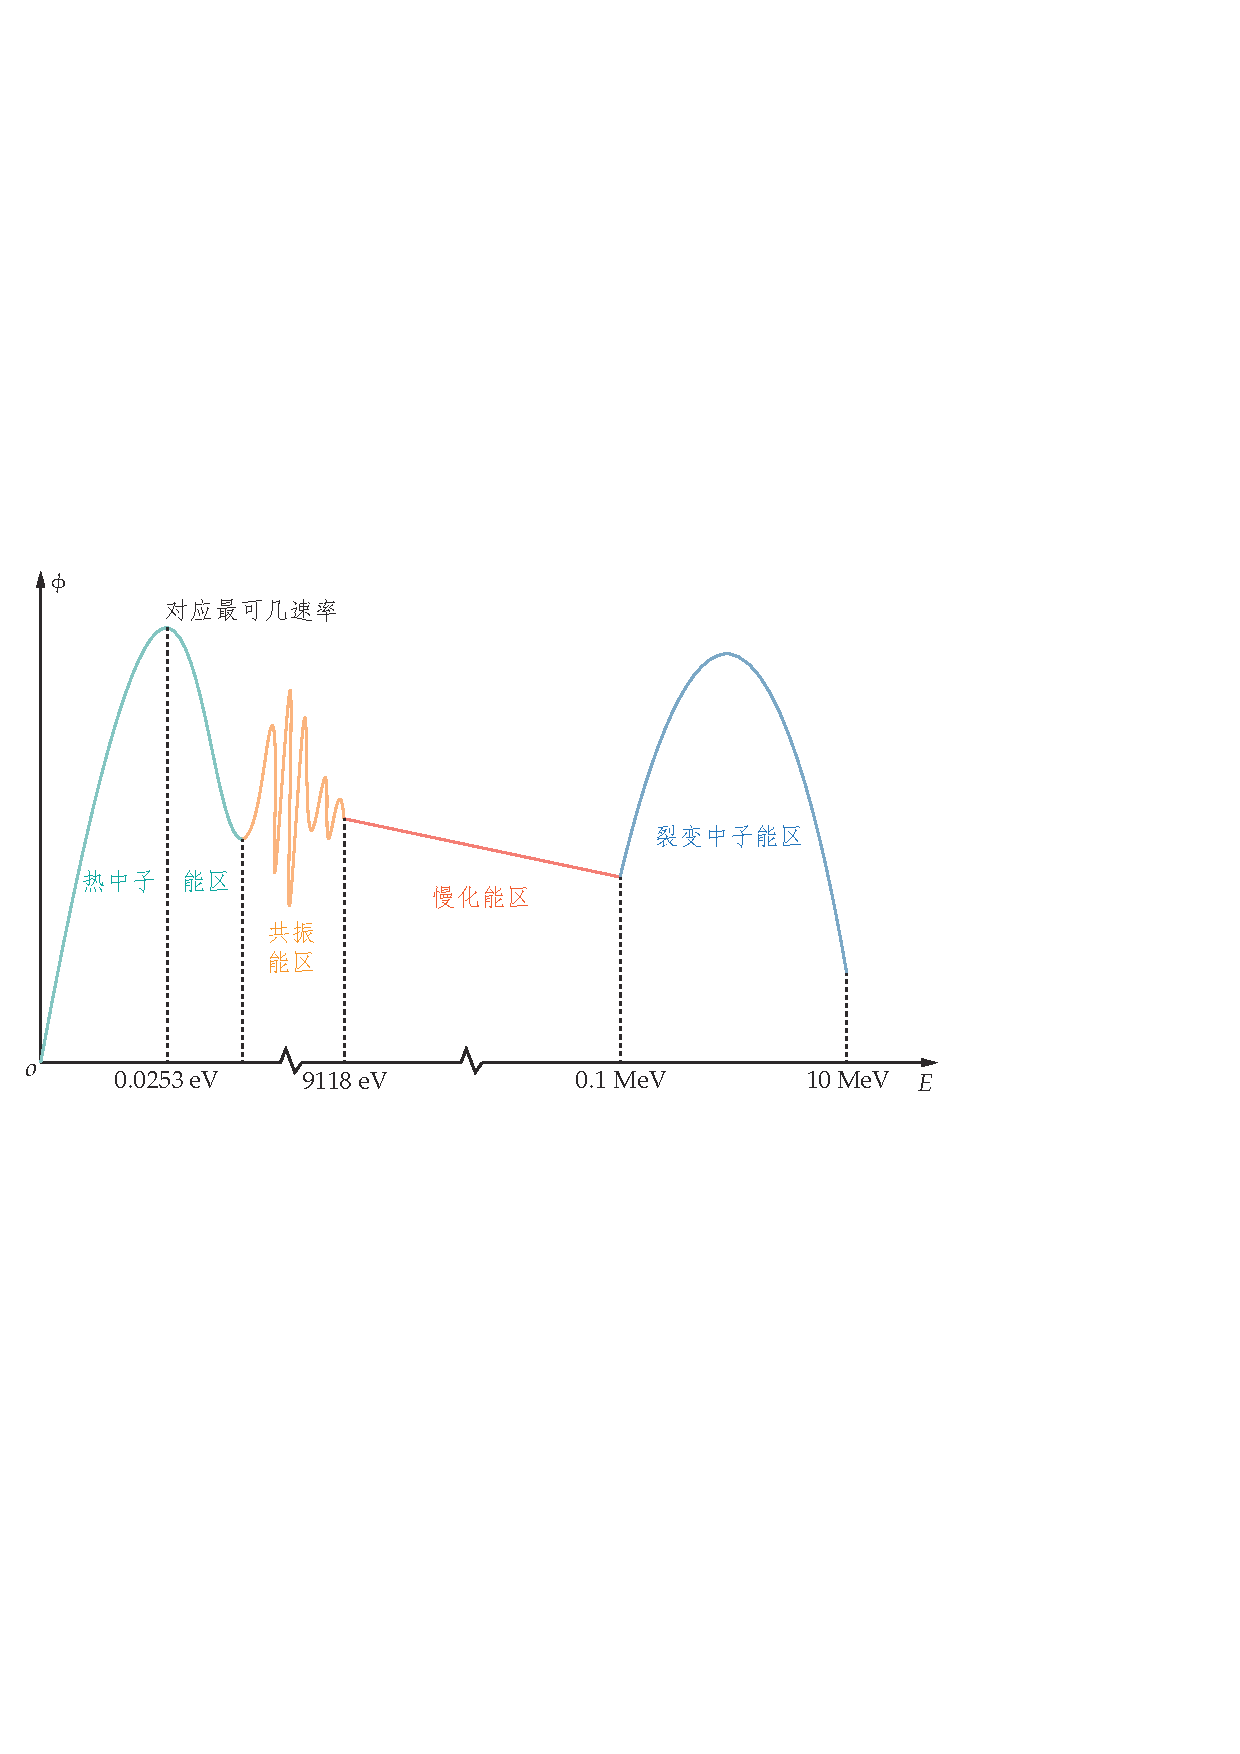
\includegraphics[scale=0.6]{figures/fig5.1.pdf}
        \end{figure}
        \begin{enumerate}[(1)]
            \item 0.1 MeV \textasciitilde \, 10 MeV:\,裂变中子能谱,\,包括瞬发中子和缓发中子;\,
            \item 9118 eV \textasciitilde \, 0.1 MeV:\,共振现象非常复杂以致不可分辨,\,近似用直线描述平均作用;\,
            \item 0 \textasciitilde \, 9118 eV:\,热中子和超热中子区,\,共振峰可辨,\,$E=0.0253\,\symrm{MeV}$对应中子最可几速率.\,
        \end{enumerate}
    \end{solution}
\end{exercise}

\begin{exercise}
    什么是首次飞行逃脱概率?\,什么是丹可夫效应?\,
    \begin{solution}
        \begin{enumerate}[(1)]
            \item 首次飞行逃脱概率:\,在燃料芯块内产生的均匀和各向同性分布的,\,能量为$E$的中子未经碰撞逃出芯块在慢化剂内发生首次碰撞的概率,\,用$P_0(E)$表示;\,
            \item 丹可夫效应:\,中子逸出燃料芯块后不一定在慢化剂中发生下一次碰撞,\,也有可能在相邻燃料芯块中发生碰撞,\,这种相邻燃料棒间的相互影响称为丹可夫效应.\,
        \end{enumerate}
    \end{solution}
\end{exercise}

\begin{exercise}
    试列出至少四种共振计算方法.\,
    \begin{solution}
        \begin{enumerate}[(1)]
            \item 窄共振近似;
            \item 无限质量近似;
            \item 中间近似;
            \item 有理近似.
        \end{enumerate}
    \end{solution}
\end{exercise}

\begin{exercise}
    什么是能量自屏效应和空间自屏效应?\,
    \begin{solution}
        \begin{enumerate}[(1)]
            \item 能量自屏效应:\,如果没有共振峰,\,慢化中子能谱近似服从$1/E$分布,\,但遇到某一共振峰时,\,由于共振核素吸收截面极大,\,$\varphi_{\symrm{R}}(E)$将会变得很小,\,从而$1/E$曲线在共振峰处出现急剧下降;\,
            \item 空间自屏效应:\,由于燃料棒中${}^{238}\symrm{U}$对超热中子具有很强的共振吸收,\,使得慢化剂中产生的超热中子刚进入到燃料表面就被吸收,\,超热中子几乎没有机会进入燃料棒内部,\,即燃料外层对内层有屏蔽作用.\,
        \end{enumerate}
    \end{solution}
\end{exercise}

\begin{exercise}
    压水堆中栅格的非均匀效应会影响到四因子模型中的哪些参数?\,作用机制是什么?\,
    \begin{solution}
        \begin{equation*}
            k_{\infty} = \highlight{NavyBlue}{\color{black} $\varepsilon$} {\color{NavyBlue!40} \uparrow} \highlight{Bittersweet}{\color{black} $p$} {\color{Bittersweet!40} \uparrow \uparrow} \highlight{xkcdHunterGreen} {\color{black} $f$} {\color{xkcdHunterGreen!40} \downarrow} \eta
        \end{equation*}
        \begin{enumerate}[(1)]
            \item 快中子在燃料棒内裂变产生,\,其在燃料块中分布高于慢化剂中,\,将增加${}^{238}\symrm{U}$裂变可能性,\,则快中子倍增系数\highlight{NavyBlue}{\color{black} $\varepsilon$}\,{\color{NavyBlue!40} $\uparrow$};
            \item 由于空间自屏效应的存在,\,超热中子几乎没有机会进入燃料棒内部,\,则燃料棒内部对超热中子的共振吸收减少,\,逃脱共振吸收概率\highlight{Bittersweet}{\color{black} $p$} {\color{Bittersweet!40} $\uparrow$};
            \item 经过充分慢化,\,中子能量可能越过共振吸收段,\,逃脱共振吸收概率\highlight{Bittersweet}{\color{black} $p$} {\color{Bittersweet!40} $\uparrow$};
            \item 热中子在慢化剂中产生,\,其在慢化剂中分布高于燃料棒中,\,燃料吸收热中子的概率减小,\,热中子利用系数\highlight{xkcdHunterGreen} {\color{black} $f$} {\color{xkcdHunterGreen!40} $\downarrow$}.
        \end{enumerate}
    \end{solution}
\end{exercise}

\begin{exercise}
    什么是过慢化和欠慢化?\,
    \begin{solution}
        \begin{enumerate}[(1)]
            \item 过慢化:\,$k_{\infty}$最大值对应的水-铀比右侧为过慢化区,\,这里慢化剂偏多,\,中子完全慢化,\,多出的慢化剂导致中子吸收增加;\,
            \item 欠慢化:\,$k_{\infty}$最大值对应的水-铀比左侧为欠慢化区,\,这里慢化剂偏少,\,中子未完全慢化,\,${}^{238}\symrm{U}$的共振吸收变大.\,
        \end{enumerate}
    \end{solution}
\end{exercise}